\section{数据结构}
\SubsecWithAuthor{ST表}{woquneidi}
\lstinputlisting[style=cppstyle]{\detokenize{src/数据结构/ST表@woquneidi.cpp}}
\subsection{线段树}
\SubsubsecWithAuthor{区间修改线段树}{woquneidi}
\lstinputlisting[style=cppstyle]{\detokenize{src/数据结构/线段树/区间修改线段树@woquneidi.cpp}}
\SubsubsecWithAuthor{线段树(初始赋值+单点修改+查找前驱后继)}{woquneidi}
\lstinputlisting[style=cppstyle]{\detokenize{src/数据结构/线段树/线段树(初始赋值+单点修改+查找前驱后继)@woquneidi.cpp}}
\SubsubsecWithAuthor{线段树}{amazy}
\lstinputlisting[style=cppstyle]{\detokenize{src/数据结构/线段树/线段树@amazy.cpp}}
\subsection{树状数组}
\SubsubsecWithAuthor{树状数组(区间修改 + 查询)}{amazy}
\lstinputlisting[style=cppstyle]{\detokenize{src/数据结构/树状数组/树状数组(区间修改 + 查询)@amazy.cpp}}
\SubsubsecWithAuthor{树状数组(单点修改 + 区间查询 + 第k小值)}{woquneidi}
\lstinputlisting[style=cppstyle]{\detokenize{src/数据结构/树状数组/树状数组(单点修改 + 区间查询 + 第k小值)@woquneidi.cpp}}
\subsection{平衡树}
\SubsubsecWithAuthor{treap}{amazy}
\lstinputlisting[style=cppstyle]{\detokenize{src/数据结构/平衡树/treap@amazy.cpp}}
\subsection{其他}
\SubsubsecWithAuthor{并查集}{amazy}
\lstinputlisting[style=cppstyle]{\detokenize{src/数据结构/其他/并查集@amazy.cpp}}
\SubsubsecWithAuthor{珂朵莉}{amazy}
\lstinputlisting[style=cppstyle]{\detokenize{src/数据结构/其他/珂朵莉@amazy.cpp}}
\section{图论}
\subsection{2-SAT}
\SubsubsecWithAuthor{2-SAT}{Song4u}
\lstinputlisting[style=cppstyle]{\detokenize{src/图论/2-SAT/2-SAT@Song4u.cpp}}
\subsection{二分图}
\SubsubsecWithAuthor{二分图最大匹配}{Song4u}
\lstinputlisting[style=cppstyle]{\detokenize{src/图论/二分图/二分图最大匹配@Song4u.cpp}}
\SubsubsecWithAuthor{二分图最大匹配}{amazy}
\lstinputlisting[style=cppstyle]{\detokenize{src/图论/二分图/二分图最大匹配@amazy.cpp}}
\SubsubsecWithAuthor{二分图最大权值匹配}{Song4u}
\lstinputlisting[style=cppstyle]{\detokenize{src/图论/二分图/二分图最大权值匹配@Song4u.cpp}}
\SubsubsecWithAuthor{匈牙利算法}{woquneidi}
\lstinputlisting[style=cppstyle]{\detokenize{src/图论/二分图/匈牙利算法@woquneidi.cpp}}
\subsection{最小生成树}
\SubsubsecWithAuthor{Boruvka}{Song4u}
\lstinputlisting[style=cppstyle]{\detokenize{src/图论/最小生成树/Boruvka@Song4u.cpp}}
\SubsubsecWithAuthor{kruskal}{Song4u}
\lstinputlisting[style=cppstyle]{\detokenize{src/图论/最小生成树/kruskal@Song4u.cpp}}
\SubsubsecWithAuthor{prim}{Song4u}
\lstinputlisting[style=cppstyle]{\detokenize{src/图论/最小生成树/prim@Song4u.cpp}}
\subsection{最短路}
\SubsubsecWithAuthor{Bellman ford}{Song4u}
\lstinputlisting[style=cppstyle]{\detokenize{src/图论/最短路/Bellman_ford@Song4u.cpp}}
\SubsubsecWithAuthor{Floyd}{Song4u}
\lstinputlisting[style=cppstyle]{\detokenize{src/图论/最短路/Floyd@Song4u.cpp}}
\SubsubsecWithAuthor{dijkstra}{Song4u}
\lstinputlisting[style=cppstyle]{\detokenize{src/图论/最短路/dijkstra@Song4u.cpp}}
\SubsubsecWithAuthor{spfa}{Song4u}
\lstinputlisting[style=cppstyle]{\detokenize{src/图论/最短路/spfa@Song4u.cpp}}
\subsection{树上算法}
\SubsubsecWithAuthor{扩展树链剖分}{amazy}
\lstinputlisting[style=cppstyle]{\detokenize{src/图论/树上算法/扩展树链剖分@amazy.cpp}}
\SubsubsecWithAuthor{树链剖分}{amazy}
\lstinputlisting[style=cppstyle]{\detokenize{src/图论/树上算法/树链剖分@amazy.cpp}}
\subsection{网络流}
\SubsubsecWithAuthor{dinic求最大流}{woquneidi}
\lstinputlisting[style=cppstyle]{\detokenize{src/图论/网络流/dinic求最大流@woquneidi.cpp}}
\SubsubsecWithAuthor{最大流最小费用}{woquneidi}
\lstinputlisting[style=cppstyle]{\detokenize{src/图论/网络流/最大流最小费用@woquneidi.cpp}}
\subsection{连通性(Tarjan)}
\SubsubsecWithAuthor{tarjan SCC缩点}{Song4u}
\lstinputlisting[style=cppstyle]{\detokenize{src/图论/连通性(Tarjan)/tarjan SCC缩点@Song4u.cpp}}
\SubsubsecWithAuthor{tarjan割点}{woquneidi}
\lstinputlisting[style=cppstyle]{\detokenize{src/图论/连通性(Tarjan)/tarjan割点@woquneidi.cpp}}
\SubsubsecWithAuthor{tarjan求eDCC}{Song4u}
\lstinputlisting[style=cppstyle]{\detokenize{src/图论/连通性(Tarjan)/tarjan求eDCC@Song4u.cpp}}
\SubsubsecWithAuthor{tarjan求vDCC}{Song4u}
\lstinputlisting[style=cppstyle]{\detokenize{src/图论/连通性(Tarjan)/tarjan求vDCC@Song4u.cpp}}
\SubsubsecWithAuthor{tarjan求强连通分量}{woquneidi}
\lstinputlisting[style=cppstyle]{\detokenize{src/图论/连通性(Tarjan)/tarjan求强连通分量@woquneidi.cpp}}
\SubsubsecWithAuthor{tarjan求边双连通分量}{woquneidi}
\lstinputlisting[style=cppstyle]{\detokenize{src/图论/连通性(Tarjan)/tarjan求边双连通分量@woquneidi.cpp}}
\SubsubsecWithAuthor{强连通分量}{amazy}
\lstinputlisting[style=cppstyle]{\detokenize{src/图论/连通性(Tarjan)/强连通分量@amazy.cpp}}
\SubsubsecWithAuthor{边双连通分量}{amazy}
\lstinputlisting[style=cppstyle]{\detokenize{src/图论/连通性(Tarjan)/边双连通分量@amazy.cpp}}
\section{数学}
\subsection{多项式}
\SubsubsecWithAuthor{FFT}{amazy}
\lstinputlisting[style=cppstyle]{\detokenize{src/数学/多项式/FFT@amazy.cpp}}
\SubsubsecWithAuthor{FWT}{amazy}
\lstinputlisting[style=cppstyle]{\detokenize{src/数学/多项式/FWT@amazy.cpp}}
\SubsubsecWithAuthor{MTT}{amazy}
\lstinputlisting[style=cppstyle]{\detokenize{src/数学/多项式/MTT@amazy.cpp}}
\SubsubsecWithAuthor{NTT}{amazy}
\lstinputlisting[style=cppstyle]{\detokenize{src/数学/多项式/NTT@amazy.cpp}}
\subsection{数论}
\SubsubsecWithAuthor{二次剩余}{amazy}
\lstinputlisting[style=cppstyle]{\detokenize{src/数学/数论/二次剩余@amazy.cpp}}
\SubsubsecWithAuthor{扩展欧几里得}{woquneidi}
\lstinputlisting[style=cppstyle]{\detokenize{src/数学/数论/扩展欧几里得@woquneidi.cpp}}
\SubsubsecWithAuthor{线性筛}{amazy}
\lstinputlisting[style=cppstyle]{\detokenize{src/数学/数论/线性筛@amazy.cpp}}
\subsection{线性代数}
\SubsubsecWithAuthor{矩阵快速幂}{amazy}
\lstinputlisting[style=cppstyle]{\detokenize{src/数学/线性代数/矩阵快速幂@amazy.cpp}}
\SubsubsecWithAuthor{线性基}{amazy}
\lstinputlisting[style=cppstyle]{\detokenize{src/数学/线性代数/线性基@amazy.cpp}}
\subsection{组合数学}
\SubsubsecWithAuthor{组合数}{amazy}
\lstinputlisting[style=cppstyle]{\detokenize{src/数学/组合数学/组合数@amazy.cpp}}
\SubsubsecWithAuthor{组合数}{woquneidi}
\lstinputlisting[style=cppstyle]{\detokenize{src/数学/组合数学/组合数@woquneidi.cpp}}
\section{字符串}
\subsection{回文串}
\SubsubsecWithAuthor{回文自动机}{amazy}
\lstinputlisting[style=cppstyle]{\detokenize{src/字符串/回文串/回文自动机@amazy.cpp}}
\SubsubsecWithAuthor{马拉车}{amazy}
\lstinputlisting[style=cppstyle]{\detokenize{src/字符串/回文串/马拉车@amazy.cpp}}
\subsection{字典树}
\SubsubsecWithAuthor{01字典树}{amazy}
\lstinputlisting[style=cppstyle]{\detokenize{src/字符串/字典树/01字典树@amazy.cpp}}
\SubsubsecWithAuthor{字典树}{amazy}
\lstinputlisting[style=cppstyle]{\detokenize{src/字符串/字典树/字典树@amazy.cpp}}
\SubsubsecWithAuthor{字典树}{woquneidi}
\lstinputlisting[style=cppstyle]{\detokenize{src/字符串/字典树/字典树@woquneidi.cpp}}
\subsection{字符串哈希}
\SubsubsecWithAuthor{字符串哈希}{amazy}
\lstinputlisting[style=cppstyle]{\detokenize{src/字符串/字符串哈希/字符串哈希@amazy.cpp}}
\subsection{字符匹配}
\SubsubsecWithAuthor{AC自动机}{amazy}
\lstinputlisting[style=cppstyle]{\detokenize{src/字符串/字符匹配/AC自动机@amazy.cpp}}
\SubsubsecWithAuthor{KMP}{woquneidi}
\lstinputlisting[style=cppstyle]{\detokenize{src/字符串/字符匹配/KMP@woquneidi.cpp}}
\SubsubsecWithAuthor{扩展KMP}{amazy}
\lstinputlisting[style=cppstyle]{\detokenize{src/字符串/字符匹配/扩展KMP@amazy.cpp}}
\section{计算几何}
\SubsecWithAuthor{凸包}{Song4u}
\lstinputlisting[style=cppstyle]{\detokenize{src/计算几何/凸包@Song4u.cpp}}
\section{杂项}
\SubsecWithAuthor{int128}{amazy}
\lstinputlisting[style=cppstyle]{\detokenize{src/杂项/int128@amazy.cpp}}
\SubsecWithAuthor{二分 三分}{Song4u}
\lstinputlisting[style=cppstyle]{\detokenize{src/杂项/二分_三分@Song4u.cpp}}
\subsection{基姆拉尔森公式}
\lstinputlisting[style=cppstyle]{\detokenize{src/杂项/基姆拉尔森公式.cpp}}
\section{附录}
\subsection{数学公式}
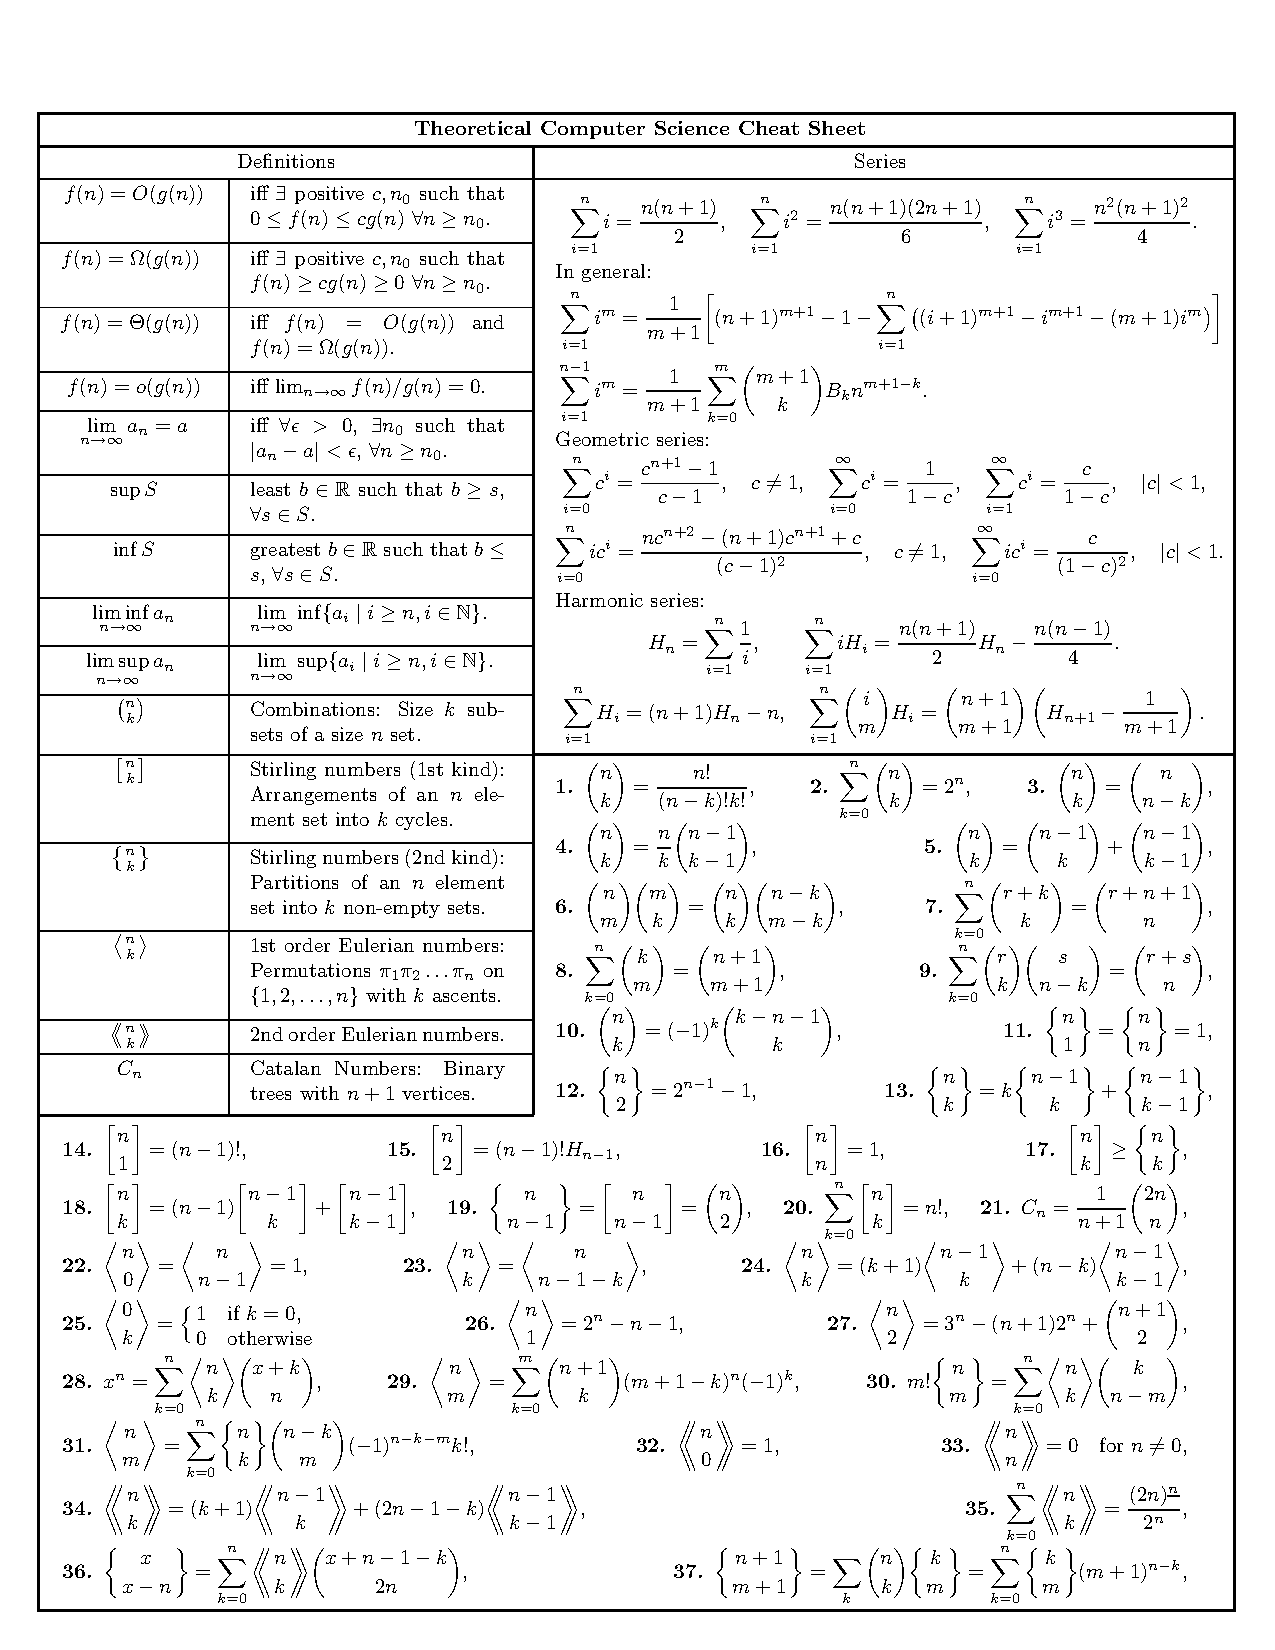
\includepdf[
  pages=-,
  angle=270,            % 旋转“内容”(逻辑页)
  width=\textwidth,    % 旋转后按版心宽度等比缩放
  pagecommand={}
]{src/附录/数学公式.pdf}
\subsection{常见错因}
爆数据(爆int, 爆longlong)\\
取mod没有取干净或者取mod时超范围\\
想不出题事算一下各种数据范围\\
}
\subsection{互质的规律}
\small {
\textbf{互质规律:}比较常见的定义
1.较大数是质数, 两个数互质

2.较小数是质数, 较大数不是它的倍数, 两个数互质

3. 1与其他数互质

4. 2与奇数互质

一些推论
1. 两个相邻的自然数一定互质

2.两个相邻的奇数一定互质

3. n与2n + 1或2n - 1一定互质

求差判断法
如果两个数相差不大,可先求出它们的差,再看差与其中较小数是否互质。如果互质,则原来两个数一定是互质数。如:194和201,先求出它们的差,201-194=7,因7和194互质,则194和201是互质数。相反也成立, 对较大数也成立

求商判断法
用大数除以小数,如果除得的余数与其中较小数互质,则原来两个数是互质数。如:317和52,317÷52=6……5,因余数5与52互质,则317和52是互质数。\\

}}
\subsection{常数表}
\begin{center}
    \begin{tabular}{|r|r|r|r|r|r|}
        \hline
        \rowcolor{gray!20}
        $n$         & $\log_{10}n$  & $n!$          & $C(n,n/2)$    & $\mathrm{LCM}(1...n)$ & $P_n$         \\ \hline
        2           & 0.30102999    & 2             & 2             & 2                     & 2             \\ \hline
        3           & 0.47712125    & 6             & 3             & 6                     & 3             \\ \hline
        4           & 0.60205999    & 24            & 6             & 12                    & 5             \\ \hline
        5           & 0.69897000    & 120           & 10            & 60                    & 7             \\ \hline
        6           & 0.77815125    & 720           & 20            & 60                    & 11            \\ \hline
        7           & 0.84509804    & 5040          & 35            & 420                   & 15            \\ \hline
        8           & 0.90308998    & 40320         & 70            & 840                   & 22            \\ \hline
        9           & 0.95424251    & 362880        & 126           & 2520                  & 30            \\ \hline
        10          & 1.00000000    & 3628800       & 252           & 2520                  & 42            \\ \hline
        11          & 1.04139269    & 39916800      & 462           & 27720                 & 56            \\ \hline
        12          & 1.07918125    & 479001600     & 924           & 27720                 & 77            \\ \hline
        15          & 1.17609126    & 1.31e12       & 6435          & 360360                & 176           \\ \hline
        20          & 1.30103000    & 2.43e18       & 184756        & 232792560             & 627           \\ \hline
        25          & 1.39794001    & 1.55e25       & 5200300       & 26771144400           & 1958          \\ \hline
        30          & 1.47712125    & 2.65e32       & 155117520     & 1.444e14              & 5604          \\ \hline
        $P_n$       & $37338_{40}$  & $204226_{50}$ & $966467_{60}$ & $190569292_{100}$     & $1e9_{114}$   \\ \hline
    \end{tabular}\\
\end{center}
\begin{center}
    $\max\omega(n)$:小于等于n中的数最大质因数个数\\
    $\max d(n)$:小于等于n中的数最大因数个数\\
    $\pi(n)$:小于等于n中的数最大互质数个数\\
    \begin{tabular}{|r|r|r|r|r|r|r|}
        \hline
        \rowcolor{gray!20}
        $n\leq$         & 10        & 100       & 1e3       & 1e4       & 1e5       & 1e6           \\ \hline
        $\max\omega(n)$ & 2         & 3         & 4         & 5         & 6         & 7             \\ \hline
        $\max d(n)$     & 4         & 12        & 32        & 64        & 128       & 240           \\ \hline
        $\pi(n)$        & 4         & 25        & 168       & 1229      & 9592      & 78498         \\ \hline
        \rowcolor{gray!20}
        $n\leq$         & 1e7       & 1e8       & 1e9       & 1e10      & 1e11      & 1e12          \\ \hline
        $\max\omega(n)$ & 8         & 8         & 9         & 10        & 10        & 11            \\ \hline
        $\max d(n)$     & 448       & 768       & 1344      & 2304      & 4032      & 6720          \\ \hline
        $\pi(n)$        & 664579    & 5761455   & 5.08e7    & 4.55e8    & 4.12e9    & 3.7e10        \\ \hline
        \rowcolor{gray!20}
        $n\leq$         & 1e13      & 1e14      & 1e15      & 1e16      & 1e17      & 1e18          \\ \hline
        $\max\omega(n)$ & 12        & 12        & 13        & 13        & 14        & 15            \\ \hline
        $\max d(n)$     & 10752     & 17280     & 26880     & 41472     & 64512     & 103680        \\ \hline
        $\pi(n)$        & \multicolumn{5}{l}{Prime number theorem: $\pi(x) \sim \frac{x}{\log(x)}$}&\\ \hline
    \end{tabular}
\end{center}}
\subsection{斐波那契数列}
\begin{enumerate}
  \item \(\displaystyle \sum_{i=1}^{n} F_i \;=\; F_{n+2}-1.\)

  \item \(\displaystyle \sum_{i=1}^{n} F_{2i-1} \;=\; F_{2n}.\)

  \item \(\displaystyle \sum_{i=1}^{n} F_{2i} \;=\; F_{2n+1}-1.\)

  \item \(\displaystyle \sum_{i=1}^{n} F_i^{2} \;=\; F_n\,F_{n+1}.\)

  \item \(\displaystyle F_{n+m} \;=\; F_{n+1}F_m \;+\; F_nF_{m-1}.\)

  \item \(\displaystyle F_{n-1}F_{n+1}-F_n^{2} \;=\; (-1)^{n}.\) \hfill(Cassini 恒等式)

  \item \(\displaystyle F_{2n-1} \;=\; F_{n}^{2}+F_{n-1}^{2}.\)

  \item \(\displaystyle F_{n} \;=\; \frac{F_{n+2}+F_{n-2}}{3}.\)

  \item \(\displaystyle F_{2n} \;=\; F_n\bigl(F_{n+1}+F_{n-1}\bigr).\)

  \item 对任意 \(k\in\mathbb{N}\),有 \(\;F_n \mid F_{nk}\).

  \item 若 \(F_a \mid F_b\),则 \(a\mid b\).

  \item \(\displaystyle \gcd(F_n,F_m) \;=\; F_{\gcd(n,m)}.\)

  \item \(\displaystyle F_n = \frac{1}{\sqrt{5}} \left[ \left( \frac{1+\sqrt{5}}{2} \right)^n - \left( \frac{1-\sqrt{5}}{2} \right)^n \right].\)
\end{enumerate}
}
\subsection{组合数学公式}
\textbf{性质1:}\\[8pt]
{\large $\mathrm{C}_{\mathrm{n}}^{\mathrm{m}} = \mathrm{C}_{\mathrm{n}}^{\mathrm{n} - \mathrm{m}}$}\\[12pt]
\textbf{性质2:}\\[8pt]
{\large $\mathrm{C}_{\mathrm{n} + \mathrm{m} + 1}^{\mathrm{m}} = \sum_{i = 0}^{\mathrm{m}} \mathrm{C}_{\mathrm{n} + i}^{i}$}\\[12pt]
\textbf{性质3:}\\[8pt]
{\large $\mathrm{C}_{\mathrm{n}}^{\mathrm{m}} \cdot \mathrm{C}_{\mathrm{m}}^{\mathrm{r}} = \mathrm{C}_{\mathrm{n}}^{\mathrm{r}} \cdot \mathrm{C}_{\mathrm{n} - \mathrm{r}}^{\mathrm{m} - \mathrm{r}}$}\\[12pt]
\textbf{性质4(二项式定理):}\\[8pt]
{\large $\sum_{i = 0}^{\mathrm{n}} \left( \mathrm{C}_{\mathrm{n}}^{i} \cdot x^{i} \right) = (1 + x)^{\mathrm{n}}$}\\[12pt]
{\large $\sum_{i = 0}^{\mathrm{n}} \mathrm{C}_{\mathrm{n}}^{i} = 2^{\mathrm{n}}$}\\[12pt]
\textbf{性质5:}\\[8pt]
{\large $\sum_{i = 0}^{\mathrm{n}} \left( (-1)^{i} \cdot \mathrm{C}_{\mathrm{n}}^{i} \right) = 0$}\\[12pt]
\textbf{性质6:}\\[8pt]
{\large $\mathrm{C}_{\mathrm{n}}^{0} + \mathrm{C}_{\mathrm{n}}^{2} + \cdots = \mathrm{C}_{\mathrm{n}}^{1} + \mathrm{C}_{\mathrm{n}}^{3} + \cdots = 2^{\mathrm{n} - 1}$}\\[12pt]
\textbf{性质7:}\\[8pt]
{\large $\mathrm{C}_{\mathrm{n} + \mathrm{m}}^{\mathrm{r}} = \sum_{i = 0}^{\min(\mathrm{n}, \mathrm{m}, \mathrm{r})} \left( \mathrm{C}_{\mathrm{n}}^{i} \cdot \mathrm{C}_{\mathrm{m}}^{\mathrm{r} - i} \right)$}\\[12pt]
{\large $\mathrm{C}_{\mathrm{n} + \mathrm{m}}^{\mathrm{n}} = \mathrm{C}_{\mathrm{n} + \mathrm{m}}^{\mathrm{m}} = \sum_{i = 0}^{\min(\mathrm{n}, \mathrm{m})} \left( \mathrm{C}_{\mathrm{n}}^{i} \cdot \mathrm{C}_{\mathrm{m}}^{i} \right), \quad (\mathrm{r} = \mathrm{n}\ |\ \mathrm{r} = \mathrm{m})$}\\[12pt]
\textbf{性质8:}\\[8pt]
{\large $\mathrm{m} \cdot \mathrm{C}_{\mathrm{n}}^{\mathrm{m}} = \mathrm{n} \cdot \mathrm{C}_{\mathrm{n} - 1}^{\mathrm{m} - 1}$}\\[12pt]
\textbf{性质9:}\\[8pt]
{\large $\sum_{i = 0}^{\mathrm{n}} \left( \mathrm{C}_{\mathrm{n}}^{i} \cdot i^2 \right) = \mathrm{n}(\mathrm{n} + 1) \cdot 2^{\mathrm{n} - 2}$}\\[12pt]
\textbf{性质10:}\\[8pt]
{\large $\sum_{i = 0}^{\mathrm{n}} \left( \mathrm{C}_{\mathrm{n}}^{i} \right)^2 = \mathrm{C}_{2\mathrm{n}}^{\mathrm{n}}$}\\[12pt]}
\subsection{随机素数}
979345007 986854057502126921\\
935359631 949054338673679153\\
931936021 989518940305146613\\
984974633 972090414870546877\\
984858209 956380060632801307\\
}
\subsection{编译参数}
-D\_GLIBCXX\_DEBUG : STL debugmode\\
-fsanitize=address :内存错误检查\\
-fsanitize=undefined :UB检查\\}